%!TEX root = ../main.tex

\chapter{Results}\label{cha:results}

In this chapter several fingerprints will be examined in detail.
In Section \ref{sec:tft} a breakdown of the fingerprint for TitForTat is given with an explanation of its appearance.
Section \ref{sec:GBM} shows several plots for the strategy GoByMajority, with a varying parameter.
As the parameter changes, a continuous deformation of the plot of the
fingerprint can be observed.
Finally, in Section \ref{sec:lse} we compare the underlying data for all fingerprints of strategies within Axelrod-Python.
This data is used to produce a heat plot of strategies similarity.

It may be useful to recall that a fingerprint for a strategy is produced by playing it against varying stochastic transformations of a probe.
The parameters varied are $x$ and $y$, as seen on fingerprints in this section.
High $x$ values correspond to high cooperation.
Conversely, high $y$ values correspond to high defection.
The colour at point $\hat{x}, \hat{y}$ on the plot indicates the expected value of the strategy when played against the transformation of the probe with parameters $\hat{x}, \hat{y}$.
This expected score has been approximated as outlined in Chapter \ref{cha:implementation}.



\section{Interpretation of TFT}\label{sec:tft}
TitForTat (see Section \ref{ssec:stra_titfortat} for an explanation of its behaviour) it is one of the most well known strategies for Prisoner's Dilemma.
Also, it produces a clean and easy to understand fingerprint, shown in Figure \ref{fig:TFT}, making it an ideal place to start.

\begin{figure}[hbtp!]
\centering
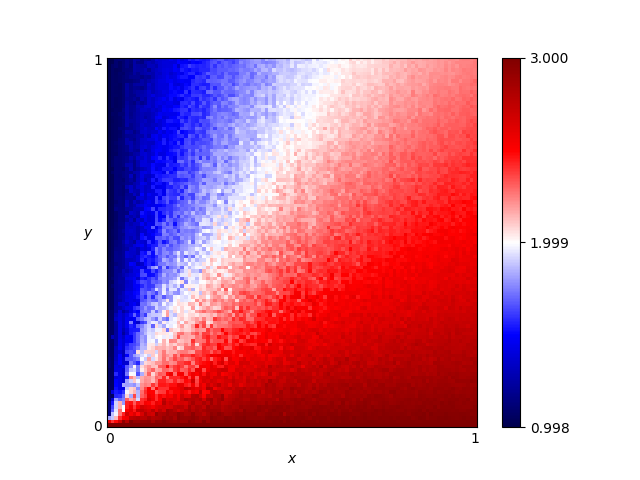
\includegraphics[width = 0.6\textwidth]{../img/Numerical/Tit_For_Tat.png}
\caption{Fingerprint for TitForTat, with TitForTat also as the probe}
\label{fig:TFT}
\end{figure}

The plot slowly transitions from a strip of blue in the top left, rotating around to a large block of red in the bottom right.
The blue area corresponds to low scores and it can be seen that this occurs for small values of $x$.
However, as $x$ increases higher scores (shown in red) quickly take over.
This is exactly as expected, TitForTat plays well in highly cooperative environments.
An immediate question is; why does the white stripe not follow the diagonal?
The main diagonal is where $x=y$ and due to the random nature of the cooperation and defections, the expected average score for TitForTat would be 2.25, slightly half the maximum possible score.
Due to the global minimum and maximum that TitForTat achieves, a score of 2.25 is not midway, and so the white line showing the middle score is off centre.



\section{Varying the parameter for Random}

It is possible to observe how changing a parameter for a strategy will affect its behaviour by comparing the fingerprints for each parameter.
As described in Section \ref{ssec:strat_random}, Random accepts a parameter that determines the probability of cooperation.
We can vary this parameter and create a new fingerprint each time.{}
In Figures \ref{fig:random0.1} to \ref{fig:random0.9} the variable is increased from 0.1 to 0.9 in steps of 0.1.
When the parameter equal 0 or 1, Random is equivalent to the strategy Defector or Cooperator respectively.
Those fingerprint plots are shown in Figures \ref{fig:rand_defect} and \ref{fig:rand_coop}.

\begin{figure}[htbp!]
\centering
\subfloat[Defector]{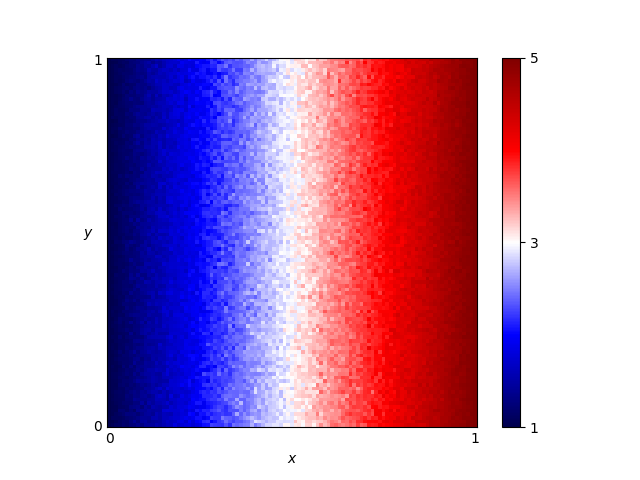
\includegraphics[width = 0.3\textwidth]{../img/Numerical/Defector.png}\label{fig:rand_defect}}\\[-2ex]

\subfloat[Random(0.1) - will cooperate\protect\\10\% of the time]{\includegraphics[width = 0.3\textwidth]{../img/Numerical/Random01.png}\label{fig:random0.1}}
\subfloat[Random(0.2) - will cooperate\protect\\20\% of the time]{\includegraphics[width = 0.3\textwidth]{../img/Numerical/Random02.png}}
\subfloat[Random(0.3) - will cooperate\protect\\30\% of the time]{\includegraphics[width = 0.3\textwidth]{../img/Numerical/Random03.png}}\\[-2ex]

\subfloat[Random(0.4) - will cooperate\protect\\40\% of the time]{\includegraphics[width = 0.3\textwidth]{../img/Numerical/Random04.png}}
\subfloat[Random(0.5) - will cooperate\protect\\50\% of the time]{\includegraphics[width = 0.3\textwidth]{../img/Numerical/Random05.png}}
\subfloat[Random(0.6) - will cooperate\protect\\60\% of the time]{\includegraphics[width = 0.3\textwidth]{../img/Numerical/Random06.png}}\\[-2ex]

\subfloat[Random(0.7) - will cooperate\protect\\70\% of the time]{\includegraphics[width = 0.3\textwidth]{../img/Numerical/Random07.png}}
\subfloat[Random(0.8) - will cooperate\protect\\80\% of the time]{\includegraphics[width = 0.3\textwidth]{../img/Numerical/Random08.png}}
\subfloat[Random(0.8) - will cooperate\protect\\90\% of the time]{\includegraphics[width = 0.3\textwidth]{../img/Numerical/Random09.png}\label{fig:random0.9}}\\

\subfloat[Cooperator]{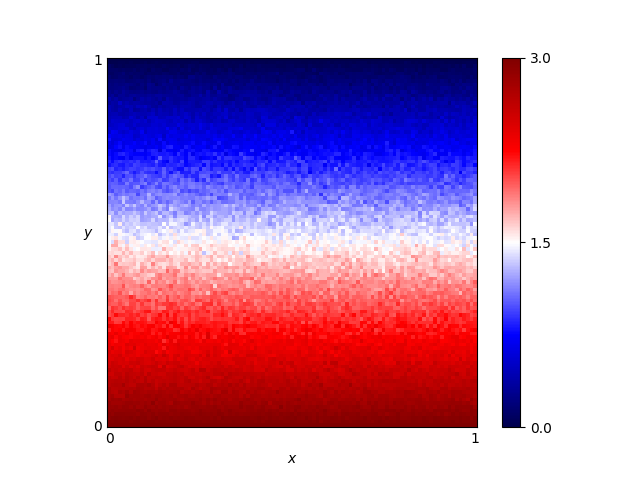
\includegraphics[width = 0.3\textwidth]{../img/Numerical/Cooperator.png}\label{fig:rand_coop}}

\end{figure}



\section{GoByMajority for different parameters}\label{sec:GBM}

Figures \ref{fig:GBM5} to \ref{fig:GBMoo} show fingerprints for the strategy GoByMajority (see section \ref{sec:fsm_proof}) with increasing memory depth when probed by TitForTat
Whilst the intricate nature of the fingerprints is hard to interpret, one major observation can be made.
As the memory depth increases, a region in the middle of the right hand side of the plot transitions from red to blue.
Blue areas correspond to lower scores, and so the strategy actually performs worse in this area when it has a larger memory.
This reason for this is not immediately apparent, and would be interesting to investigate in further research.

\begin{figure}[htbp!]
\centering
\subfloat[GoByMajority with memory \newline depth 5]{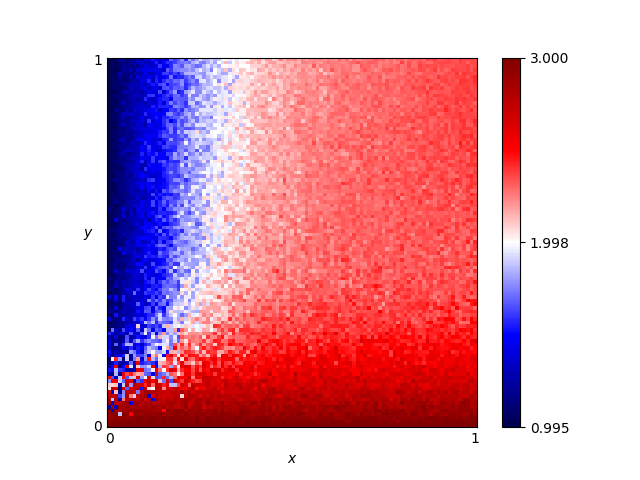
\includegraphics[width = 0.3\textwidth]{../img/Numerical/Go_By_Majority_5.png}\label{fig:GBM5}}
\subfloat[GoByMajority with memory \newline depth 10]{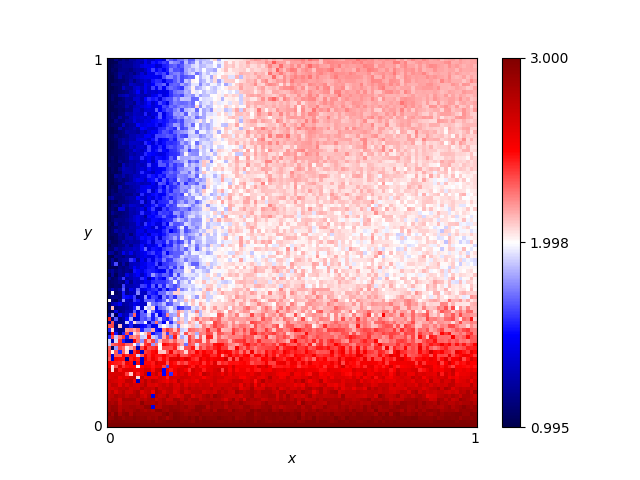
\includegraphics[width = 0.3\textwidth]{../img/Numerical/Go_By_Majority_10.png}}
\subfloat[GoByMajority with memory \newline depth 20]{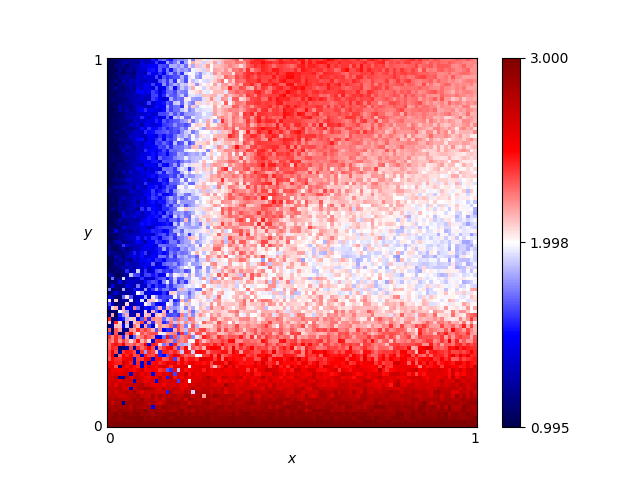
\includegraphics[width = 0.3\textwidth]{../img/Numerical/Go_By_Majority_20.png}}\\
\subfloat[GoByMajority with memory \newline depth 40]{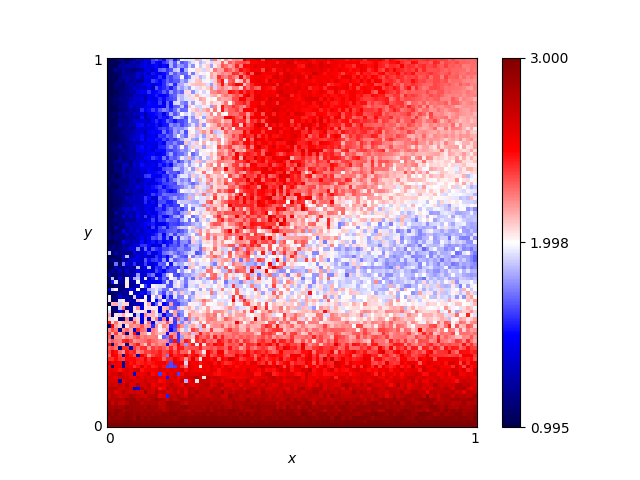
\includegraphics[width = 0.3\textwidth]{../img/Numerical/Go_By_Majority_40.png}}
\subfloat[GoByMajority with memory \newline depth 75]{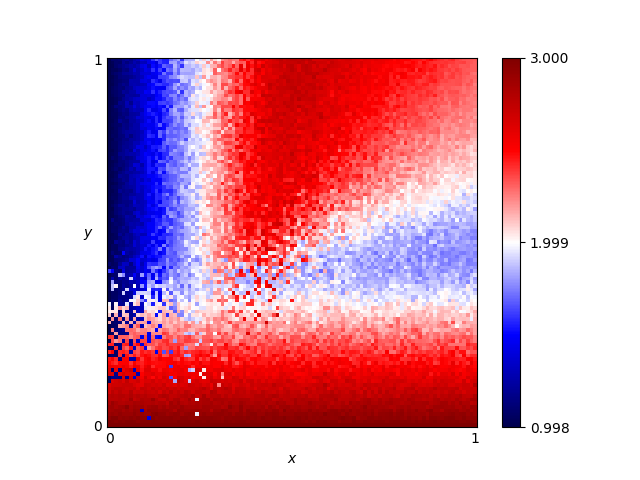
\includegraphics[width = 0.3\textwidth]{../img/Numerical/Go_By_Majority_75.png}}
\subfloat[GoByMajority with memory \newline depth infinite]{\includegraphics[width = 0.3\textwidth]{../img/Numerical/Go_By_Majority0.png}\label{fig:GBMoo}}
\end{figure}



\section{Random and Cycler(CDDC) with Different probes}

The importance of probe selection will now be demonstrated.
Thus far, all fingerprints shown have used TitForTat as a probe, but this is not always enough.
For example, Random and Cycler(CDDC) produce identical fingerprints when probed with TitForTat, as shown in \ref{fig:rand_cycle_tft}.

\begin{figure}[htbp!]
    \centering
    \subfloat[Fingerprint for Random]{\includegraphics[width = 0.5\textwidth]{../img/Numerical/Random05.png}}
    \subfloat[Fingerprint for Cycler(CDDC)]{\includegraphics[width = 0.5\textwidth]{../img/Numerical/Cycler(CDDC)_TFT.png}}
    \caption{Fingerprints for Random and Cylcer(CDDC) when probed by TitForTat}
    \label{fig:rand_cycle_tft}
\end{figure}

Even when changing the probe to TitForTwoTats or TwoTitsForTat the Fingerprints remain the same, as shown in Figures \ref{fig:rand_cycle_tf2t} and \ref{fig:rand_cycle_2tft}.

\begin{figure}[htbp!]
    \centering
    \subfloat[Fingerprint for Random]{\includegraphics[width = 0.5\textwidth]{../img/Numerical/Random_TF2T.png}}
    \subfloat[Fingerprint for Cycler(CDDC)]{\includegraphics[width = 0.5\textwidth]{../img/Numerical/Cycler(CDDC)_TF2T.png}}
    \caption{Fingerprints for Random and Cylcer(CDDC) when probed by TitForTwoTat}
    \label{fig:rand_cycle_tf2t}
\end{figure}

\begin{figure}[htbp!]
    \centering
    \subfloat[Fingerprint for Random]{\includegraphics[width = 0.5\textwidth]{../img/Numerical/Random05_2TFT.png}}
    \subfloat[Fingerprint for Cycler(CDDC)]{\includegraphics[width = 0.5\textwidth]{../img/Numerical/Cycler_CDDC_2TFT.png}}
    \caption{Fingerprints for Random and Cylcer(CDDC) when probed by TwoTitsForTat}
    \label{fig:rand_cycle_2tft}
\end{figure}

However, changing the probe to TitForThreeTats as in Figure \ref{fig:rand_cycle_tf3t}, it becomes clear that the strategies are different.
This example highlights the importance of choosing an appropriate probe when Fingerprinting.

\begin{figure}[htbp!]
    \centering
    \subfloat[Fingerprint for Random]{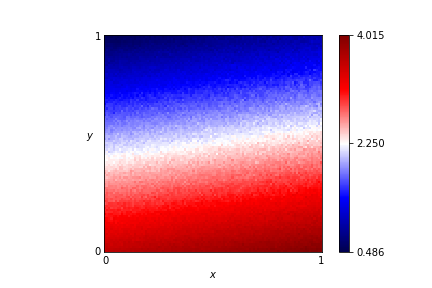
\includegraphics[width = 0.5\textwidth]{../img/Numerical/Random_TF3T.png}}
    \subfloat[Fingerprint for Cycler(CDDC)]{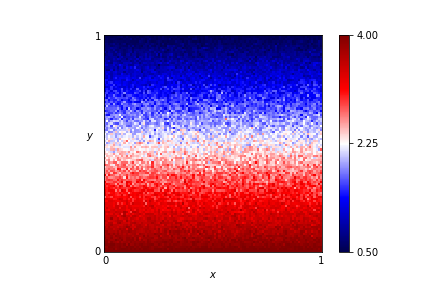
\includegraphics[width = 0.5\textwidth]{../img/Numerical/Cycler(CDDC)_TF3T.png}}
    \caption{Fingerprints for Random and Cylcer(CDDC) when probed by TitForThreeTat}
    \label{fig:rand_cycle_tf3t}
\end{figure}


\section{LSE plot and table}\label{sec:lse}
As described several times, a fingerprint for a strategy is merely the expected score when it plays against a probe with varying parameters.
All the fingerprint plots shown thus far are approximations of this, where the score for specific values of $x, y$ is calculated and then plotted.
Within Axelrod-Python all these underlying scores are recorded in a \mintinline{python}{.csv} file and can therefore be compared directly.

For two strategies $A$ and $B$ where $s_{x, y}^{(A)}$ is the score for strategy $A$ at point $x, y$ and $P_x, P_y$ are the set of points taken by $x, y$, we can compute a rudimentary value of `similarity' by calculating the Mean Square Error:
$$
\text{MSE}(A, B) = \sum_{x \in P_x} \sum_{y \in P_y} \frac{(s_{x, y}^{(A)} - s_{x, y}^{(B)})^2}{|P_x|\times|P_y|}
$$
When $\text{MSE}(A, B) \approx 0$, the two strategies $A$, $B$ are very similar, and so further investigation should be carried out between them.
After calculating $\delta(A, B)$ for all pairs of strategies, a matrix plot can then be created giving an overview of the similarity between the set of strategies.
This is shown in Figure \ref{fig:mean_squares}.

\begin{figure}[htbp!]
    \makebox[\textwidth][c]{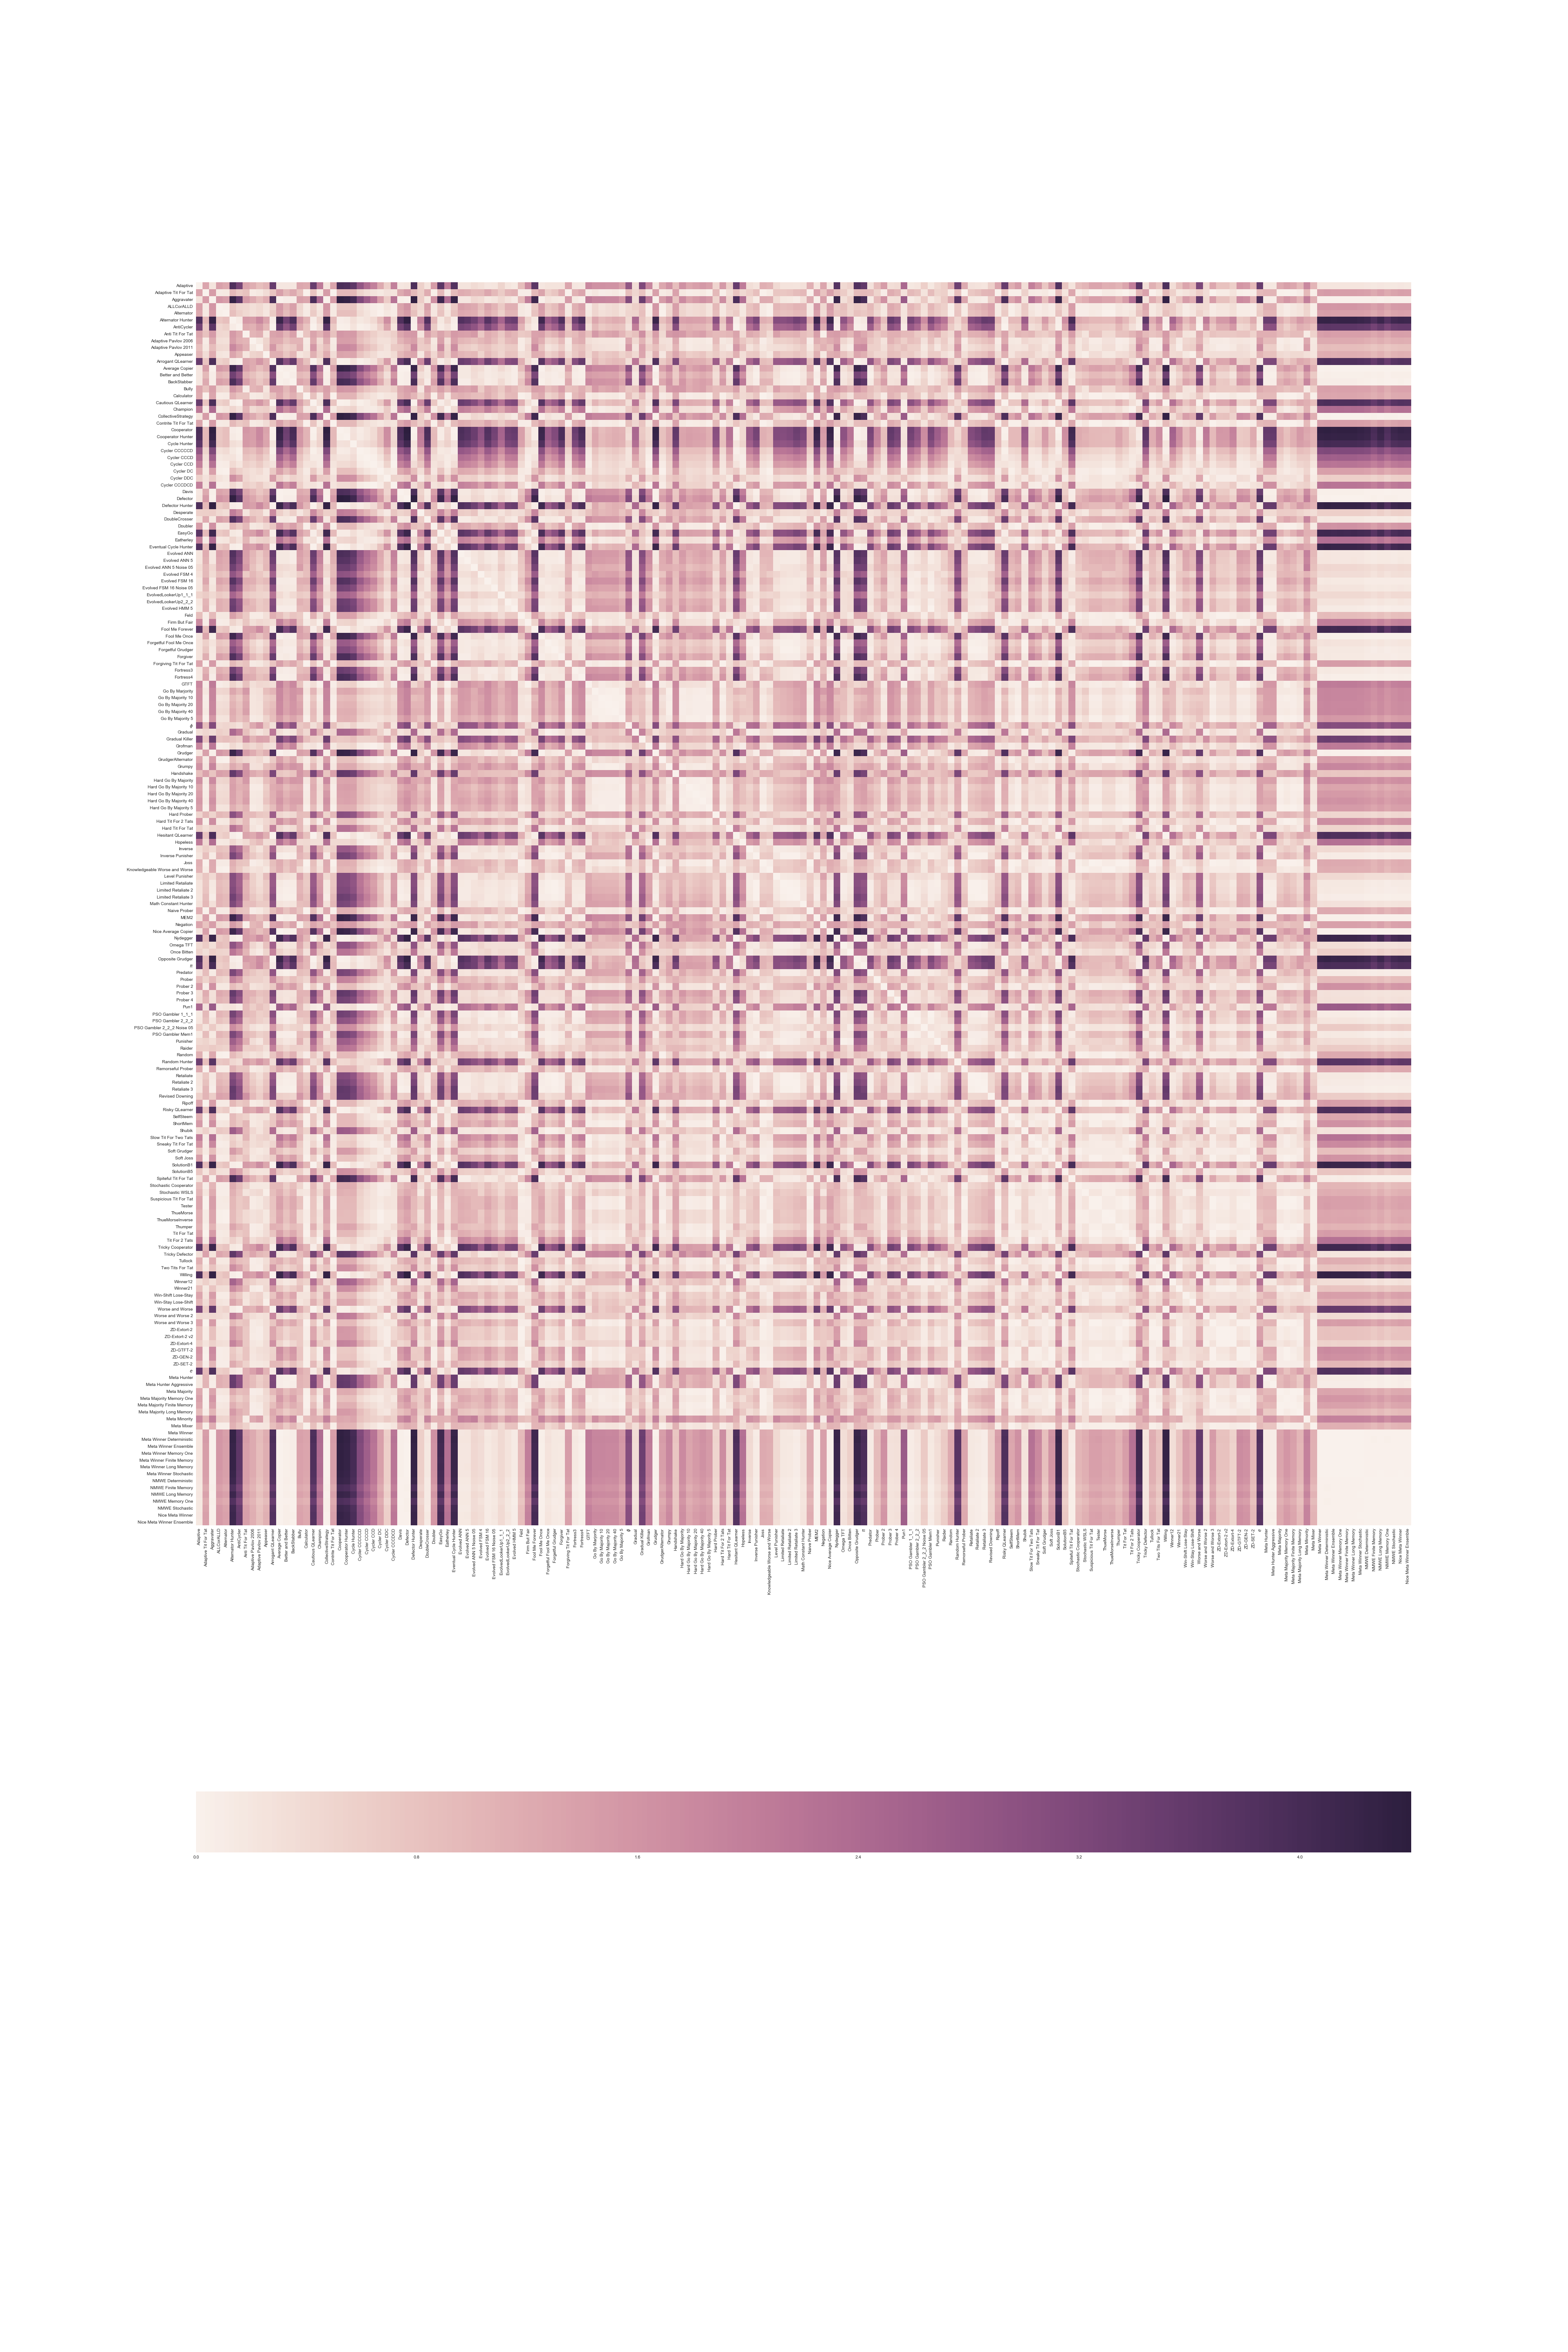
\includegraphics[width=\linewidth]{../img/mean_squares.png}}
    \caption{Caption here}
    \label{fig:mean_squares}
\end{figure}
